%! Author = zhenxiang
%! Date = 23-3-30

\PassOptionsToPackage{quiet}{xeCJK}  % 抑制无意义的警告
% Preamble
\documentclass[11pt]{ctexart}


% Packages
\usepackage{amsmath}
% graphicx
\usepackage{graphicx}
% 页面设置
\usepackage{geometry}
\geometry{left=2.5cm, right=2.5cm, top=2.5cm, bottom=2.5cm}
% codes
\usepackage{ listings}
\usepackage{xcolor}
\usepackage{color}
\definecolor{mygreen}{rgb}{0,0.6,0}
\definecolor{mygray}{rgb}{0.5,0.5,0.5}
\definecolor{mymauve}{rgb}{0.58,0,0.82}
\lstset{ %
	backgroundcolor=\color{white},   % choose the background color; you must add \usepackage{color} or \usepackage{xcolor}
	basicstyle=\ttfamily,            % the size of the fonts that are used for the code
	breakatwhitespace=false,         % sets if automatic breaks should only happen at whitespace
	breaklines=true,                 % sets automatic line breaking
	captionpos=b,                    % sets the caption-position to bottom
	commentstyle=\ttfamily\color{mygreen},    
	% comment style
	deletekeywords={},               % if you want to delete keywords from the given language
	escapeinside={},                 % if you want to add LaTeX within your code
	extendedchars=true,              % lets you use non-ASCII characters; for 8-bits encodings only, does not work with UTF-8
	frame=single,                    % adds a frame around the code
	keepspaces=true,                 % keeps spaces in text, useful for keeping indentation of code (possibly needs columns=flexible)
	keywordstyle=\color{blue},       % keyword style
	language=C++,                    % the language of the code
	morekeywords={},                 % if you want to add more keywords to the set
	numbers=left,                    % where to put the line-numbers; possible values are (none, left, right)
	numbersep=5pt,                   % how far the line-numbers are from the code
	numberstyle=\tiny\color{mygray}, % the style that is used for the line-numbers
	rulecolor=\color{black},         % if not set, the frame-color may be changed on line-breaks within not-black text (e.g. comments (green here))
	showspaces=false,                % show spaces everywhere adding particular underscores; it overrides 'showstringspaces'
	showstringspaces=false,          % underline spaces within strings only
	showtabs=false,                  % show tabs within strings adding particular underscores
	stepnumber=1,                    % the step between two line-numbers. If it's 1, each line will be numbered
	stringstyle=\color{mymauve},     % string literal style
	tabsize=2,                       % sets default tabsize to 2 spaces
	title=\lstname                   % show the filename of files included with \lstinputlisting; also try caption instead of title
}

% Document
\begin{document}

\section{Reading}

\subsection{Memory and data locality}

迄今为止,我们已经学习了如何编写CUDA内核函数以及如何通过大量线程配置和协调其执行。在本章中,我们将研究如何组织和定位数据,以便大量线程可以高效地访问它们。在第二章《数据并行计算》中,我们讨论了数据首先从主机内存传输到设备全局内存。在第三章《可伸缩并行执行》中,我们确定了如何使用块索引和线程索引使线程从全局内存中访问其数据部分。我们还探索了资源分配和线程调度。虽然我们所涵盖的范围是一个很好的起点,但我们迄今学到的CUDA内核函数可能只能实现底层硬件潜在速度的一小部分。这种性能低下归因于全局内存的长延迟(数百个时钟周期)和有限访问带宽,通常使用动态随机访问存储器实现。虽然有大量的线程可用于执行,理论上可以容忍长时间的内存访问延迟,但您很容易会遇到一种情况,即全局内存访问路径中的交通拥塞阻止了除少数线程以外的所有线程取得进展,从而使一些流多处理器(SMs)闲置。为了避免这种拥塞,CUDA提供了许多额外的资源和访问内存的方法,可以消除大部分与全局内存的交通。在本章中,您将学习使用不同类型的内存来提高CUDA内核函数的执行效率。

\subsubsection{IMPORTANCE OF MEMORY ACCESS EFFICIENCY}

在下面这串代码,其中\ verb|pixVal += in[curRow * w + curCol]| 这行代码,全局内存访问获取一个in[]数组元素,浮点加法操作是pixVal+=

因此浮点计算与全局内存访问操作的比率是1:1,即1.0,我们将这个比率称为计算-全局内存访问比率,它表示在程序的某个区域内执行每次访问全局内存所需执行的浮点计算数量。

计算-全局内存访问比率对CUDA内核的性能有重要影响。
In a high-end(高端) device today, the global memory bandwidth is around 1,000 GB/s, or 1 TB/s. With four bytes in each single-precision
floating-point value, no more than 1000/4 = 250 giga single-precision operands per
second can be expected to load. With a compute-to-global-memory ratio of 1.0, the
execution of the image blur kernel will be limited by the rate at which the operands
(e.g., the elements of in[]) can be delivered to the GPU. We will refer to programs
whose execution speed is limited by memory access throughput as memory-bound
programs. In our example, the kernel will achieve no more than 250 giga floating-
point operations per second (GFLOPS).

在当今高端设备中,全局内存带宽约为1,000 GB/s或1 TB/s。每个单精度浮点值占用4个字节,因此最多可以期望加载1000/4=250 giga单精度操作数每秒。如果计算-全局内存比率为1.0,则图像模糊内核的执行将受到将操作数(如in[]的元素)传输到GPU的速率的限制。我们将执行速度受内存访问吞吐量限制的程序称为内存限制程序。在我们的示例中,内核的执行速度将不会超过250 giga浮点操作每秒(GFLOPS)。
虽然250 GFLOPS是一个可观的数字,但它仅是高端设备峰值单精度性能12 TFLOPS或更高的微不足道的一部分(2\%)。为了实现更高水平的内核性能,我们需要通过减少全局内存访问的数量来增加计算-全局内存比率。要实现处理器的峰值12 TFLOPS评级,我们需要48或更高的比率。一般来说,随着计算吞吐量增长速度快于内存带宽,过去几代设备中所需的比率已经在增加。本章的其余部分介绍一种常用的减少全局内存访问次数的技术。




\begin{lstlisting}
	__global__
void blurKernel(unsigned char * in, unsigned char * out, int w, int h){
	int Col  = blockIdx.x * blockDim.x + threadIdx.x;
	int Row = blockIdx.y * blockDim.y + threadIdx.y;
	
	if (Col < w && Row < h) {
		int pixVal = 0;
		int pixels = 0;	
		// Get the average of the surrounding BLUR_SIZE x BLUR_SIZE box
		for (int blurRow = - BLUR_SIZE; blurRow < BLUR_SIZE + 1; ++blurRow) {
			int curRow = Row + blurRow;
			int curCol = Col + blurCol;
			// Verify we have a valid image pixel
			if(curRow > -1 && curRow < h && curCol > -1 && curCol < w) {
				pixVal += in[curRow * w + curCol];
				pixels++; // Keep track of number of pixels in the avg	
			}		
			
		}
	}
	// Write our new pixel value out
	out[Row * w + Col] = (unsigned char)(pixVal /pixels); 
	
}

}



\end{lstlisting}

\subsubsection{MATRIX MULTIPLICATION}



矩阵乘法,在每次迭代中,需要执行两次全局内存访问以进行一次浮点数乘法和一次浮点数加法。一次全局内存访问获取一个M元素,另一次获取一个N元素。一次浮点数操作乘以获取的M和N元素,另一次将乘积累加到Pvalue中。因此,循环的计算与全局内存访问比率为1.0。

\begin{lstlisting}
	__global__ void MatrixMulKernel(float* M, float* N, float* P,
	int Width) {
		// Calculate the row index of the P element and M
		int Row = blockIdx.y*blockDim.y+threadIdx.y;
		// Calculate the column index of P and N
		int Col = blockIdx.x*blockDim.x+threadIdx.x;
		if ((Row < Width) && (Col < Width)) {
			float Pvalue = 0;
			// each thread computes one element of the block sub-matrix
			for (int k = 0; k < Width; ++k) {
				Pvalue += M[Row*Width+k]*N[k*Width+Col];
			}
			P[Row*Width+Col] = Pvalue;
		}
	}
\end{lstlisting}


\subsubsection{CUDA MEMORY TYPES}

在CUDA设备中,有几种类型的内存可以帮助程序员提高计算与全局内存访问比率,从而实现高执行速度。

% 图片置于当前位置
\begin{figure}[ht]
	\centering
	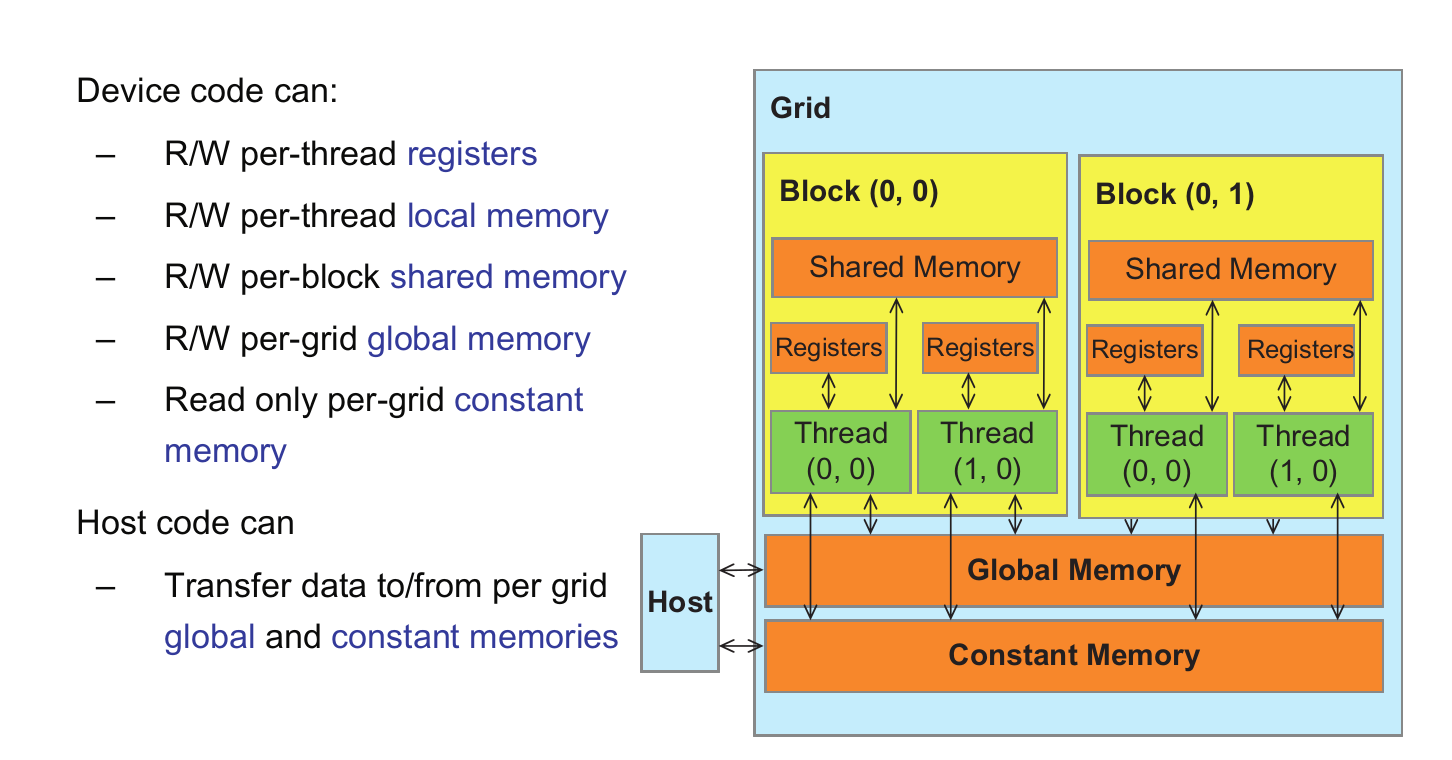
\includegraphics[width=1.0\textwidth]{images/OverviewoftheCUDAdevicememorymodel.png}
	\caption{Overview of the CUDA device memory model}
	\label{fig:1}
\end{figure}

Overview of the CUDA device memory model

\begin{itemize}
	\item 
\end{itemize}

\end{document}